\section{Análisis experimental}

Se analizaron los resultados que se obtuvieron al ejecutar las implementaciones en C++, Java y Python sobre 53 instancias, comparando los tiempos de ejecución y el comportamiento práctico.

\subsection{Solución base Backtracking}

En primera instancia se analizará los resultados obtenidos a través de la metodología backtracking con el fin de determinar las diferencias entre los enfoques mencionados con anterioridad.

\subsubsection{Resultados}

Los resultados obtenidos tras la ejecución de estas tres implementaciones se detallan a continuación mediante una tabla y gráfico comparativo.

\begin{center}
\begin{tabular}{lccc}
\toprule
Lenguaje & Tiempo Promedio (ms) & Tipo de Enfoque & Observación \\
\midrule
Java   & $\sim$10.2   & Terminación temprana & Más rápido \\
Python & $\sim$610.5  & Terminación temprana & Intermedio \\
C++    & $\sim$800.2  & Exhaustivo con poda & Más lento \\
\bottomrule
\end{tabular}
\end{center}
\small \textit{Fuente: Elaboración propia basada en los resultados obtenidos tras ejecutar tools benchmark.}

\begin{figure}[H]
\centering
\caption{Tiempo de ejecución promedio en C++, Java y Python (53 instancias).}
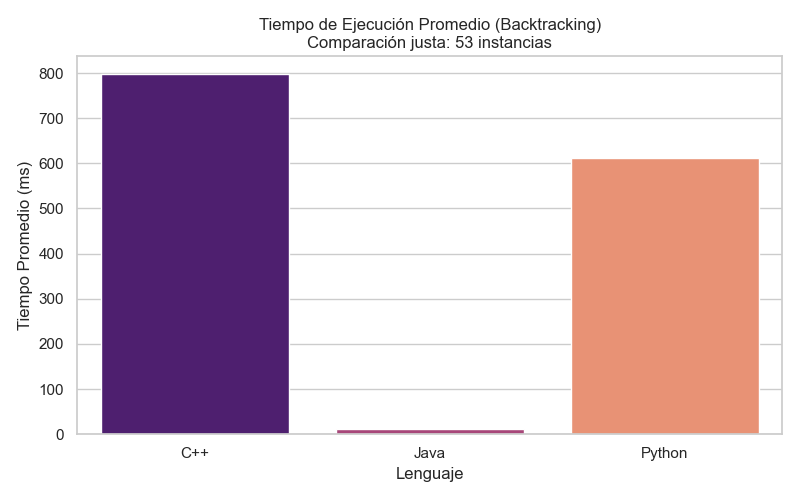
\includegraphics[width=0.8\textwidth]{figuras/backtracking_time_bar.png}
\\
\small \textit{Fuente: Elaboración propia basada en los resultados obtenidos tras ejecutar tools benchmark.}
\label{fig:tiempos}
\end{figure}

Como es posible observar en la Figura \ref{fig:tiempos}, Java presenta un menor tiempo de ejecución, seguido por Python y finalmente C++

\subsubsection{Escalabilidad}

El problema presenta complejidad exponencial por lo que todos los enfoques aumentan su tiempo de ejecución cuando crece el tamaño del grafo. Sin embargo, la terminación temprana permite a Java y Python escalar mejor en la practica.

\subsubsection{Análisis}

La principal diferencia radica en el enfoque de los algoritmos. Java y Python utilizan una estrategia de decision con terminación temprana, deteniéndose al momento de encontrar la solución óptima. Por otro lado C++ realiza una exploración mas exhaustiva, lo cual incrementa su tiempo de ejecución.

Entre Java y Python, la ventaja de la implementación de Java se debe a la optimización JIT y mejor manejo de la memoria.


% --- FIN Backtracking ---

\subsection{Solución mejorada heurísticas Greedy}

Ahora se procederá a analizar la solución mejorada que en este caso sera mediante la técnica Greedy (heurísticas avara)

\subsubsection{Resultados}

Los resultados obtenidos tras la ejecución de estas tres implementaciones se detallan a
continuación mediante una tabla y gráfico comparativo.

\begin{center}
\begin{tabular}{lccc}
\toprule
Lenguaje & Tiempo Promedio (ms) & Tipo de Enfoque & Observación \\
\midrule
C++    & $\sim$0.01  & Greedy directo        & Más rápido \\
Python & $\sim$0.09  & Greedy con ordenamiento & Intermedio \\
Java   & $\sim$0.12  & Greedy secuencial     & Más lento \\
\bottomrule
\end{tabular}
\end{center}
\small \textit{Fuente: Elaboración propia basada en los resultados obtenidos tras ejecutar tools benchmark.}

\begin{figure}[H]
\centering
\caption{Tiempo de ejecución promedio del algoritmo Greedy (53 instancias).}
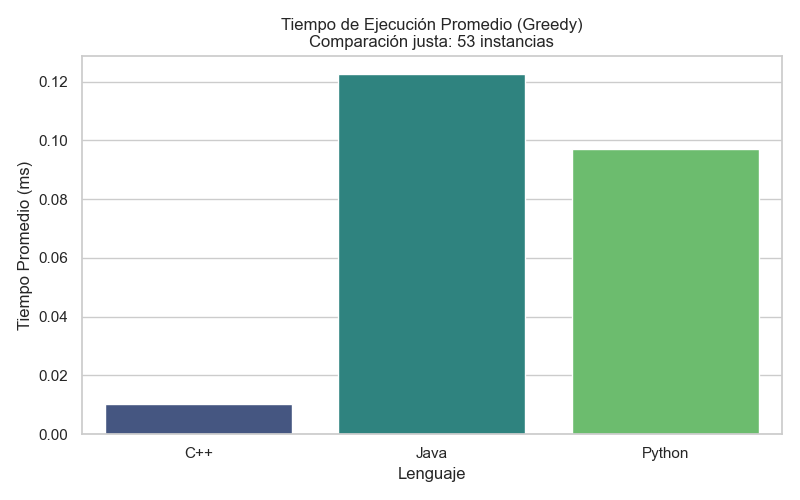
\includegraphics[width=0.7\textwidth]{figuras/greedy_time_bar.png}
\\
\small \textit{Fuente: Elaboración propia basada en los resultados obtenidos tras ejecutar tools benchmark.}
\label{fig:greedy_tiempos}
\end{figure}

Como se observa en la Figura \ref{fig:greedy_tiempos}, C++ presenta el menor tiempo, seguido por Python y Java.

\subsubsection{Escalabilidad}

En esta sección se analizará en como varía el tiempo de ejecución en función del tamaño del grafo.

\begin{figure}[H]
\centering
\caption{Tiempo de ejecución en función de la cantidad de nodos.}
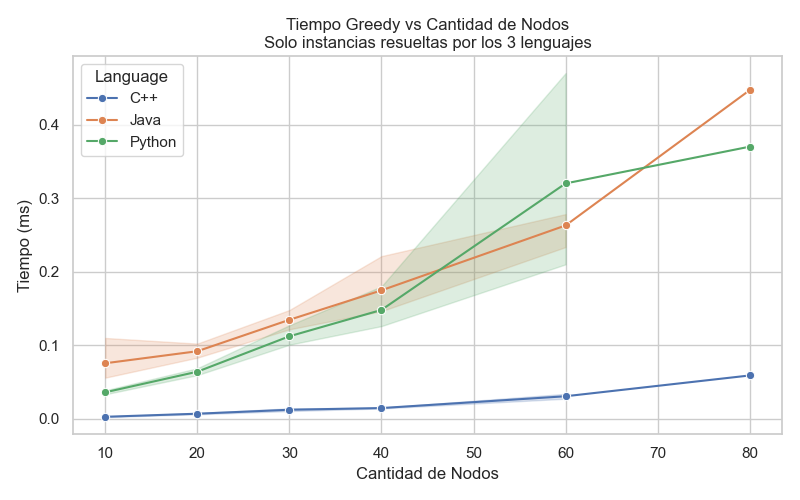
\includegraphics[width=0.8\textwidth]{figuras/greedy_time_vs_nodes.png}
\\
\small \textit{Fuente: Elaboración propia basada en los resultados obtenidos tras ejecutar tools benchmark.}
\label{fig:greedy_escalabilidad}
\end{figure}

La Figura \ref{fig:greedy_escalabilidad} muestra un crecimiento aproximadamente lineal del tiempo de ejecución en los tres lenguajes, con diferencias en la pendiente.

\subsubsection{Análisis}

Las diferencias se explican principalmente por la implementación:

\begin{itemize}
    \item C++ logra el mejor rendimiento gracias a su ejecución nativa y bajo overhead.
    \item Python mejora su desempeño mediante el ordenamiento previo, reduciendo conflictos.
    \item Java presenta mayor tiempo debido a la sobrecarga de la JVM en ejecuciones cortas.
\end{itemize}

A diferencia del backtracking, el enfoque Greedy no garantiza optimalidad, pero reduce significativamente el tiempo de ejecución al evitar la exploración exhaustiva.

\subsection{Comparación de Enfoques}

Para evaluar la calidad de las soluciones generadas por la heurísticas Greedy, se comparó el número de cliques obtenidos mediante dicha solución mejorada y el número de cliques correspondiente al algoritmo backtracking. Es importante recalcar que el objetivo que se busca con \textit{Clique Cover} es minimizar el numero de cliques, por lo que una menor diferencia espacial entre Greedy respecto a backtracking indica una heurísticas más precisa. 

\subsubsection{Análisis de Calidad de la Solución (Diferencia de Cliques)}

El siguiente gráfico ilustra la cantidad promedio de cliques adicionales que la solución Greedy genera en comparación con el óptimo teórico, tras evaluar 53 instancias.

\begin{figure}[H]
\centering
\caption{Diferencia promedio de cliques generados (Greedy vs. Backtracking Óptimo) para 53 instancias.}
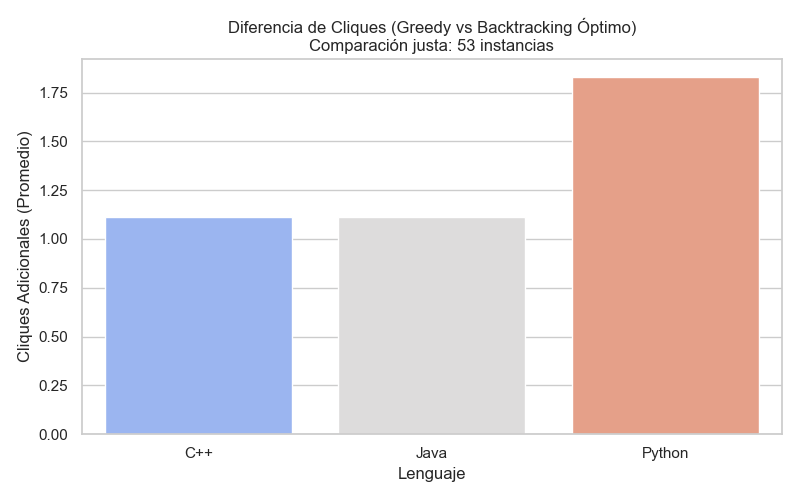
\includegraphics[width=0.8\textwidth]{figuras/quality_greedy_vs_bt.png}
\\
\small \textit{Fuente: Elaboración propia basada en los resultados obtenidos tras ejecutar tools benchmark.}
\label{fig:diff_cliques}
\end{figure}

Como es posible observar en la Figura \ref{fig:diff_cliques}, se nota la existencia de una penalización en la calidad de la solución cuando se utiliza el enfoque Greedy, la cual va variando según el lenguaje de programación y sus respectivas implementaciones de la heurística:

\begin{itemize}
    \item \textbf{C++ ($\sim$1.1 cliques adicionales):} Procesa los nodos de forma secuencial ($0$ a $n-1$). Obtiene una cota de error baja, cercana a la solución óptima.

    \item \textbf{Java ($\sim$1.1 cliques adicionales):} Presenta un comportamiento prácticamente idéntico a C++, debido a una lógica secuencial similar en el procesamiento de los vértices.

    \item \textbf{Python ($\sim$1.8 cliques adicionales):} Muestra el mayor error, a pesar de utilizar ordenamiento previo por grado, lo que no logra mejorar la calidad de la solución en estas instancias.
\end{itemize}

\subsubsection{Discusión del Compromiso Tiempo vs. Calidad}

Los resultados obtenidos logran evidenciar el clásico \textit{trade-off} en la resolución de problemas \textit{NP-completos}: 

\begin{enumerate}
    \item \textbf{Fallo de la heurística de grado (Python):} El ordenamiento por grado descendente no resulta efectivo en estas instancias, generando más cliques al fragmentar el grafo tempranamente.

    \item \textbf{Eficiencia computacional:} Aunque no se alcanza el óptimo, el tiempo se reduce drásticamente respecto a backtracking. Para escenarios donde se tolera un pequeño error, el enfoque greedy secuencial ofrece un buen balance entre calidad y rapidez.
\end{enumerate}







